
\textbf{Embedded gdagent{}}\\
\begin{itemize}
\item If you are starting your \gdaut{} and running your tests on your local machine, 
you can now connect to an embedded \gdagent{} directly from the \ite. 
\item This saves you having to start an \gdagent{} on localhost. 
\item This is also useful for testers working with \jb{} as a feature in an Eclipse installation. 
\item The embedded \gdagent{} is started on port 60000 by default; this number can be changed in the preferences.

\begin{figure}[h]
\begin{center}
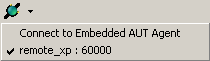
\includegraphics{52/ps/EmbeddedAgent}
\caption{Embedded AUT Agent}
\label{RNEmbeddedAgent}
\end{center}
\end{figure}


\end{itemize}

\textbf{Refactor: Replace with \gdcase{}}
\begin{itemize}
\item In the \gdtestcaseeditor{} and \gdtestsuiteeditor{}, there is a new option to replace one or more selected \gdcases{} with another \gdcase{} from the library. 
\item A new wizard takes you step-by-step through the replacement process, letting you transfer component names, match parameters and add further information for the new \gdcase{}.
\item This feature should help testers who want to restructure their tests after creating a reusable module to replace one or more \gdcases{}. 
\end{itemize}

\textbf{\gdomeditor{}: Cleanup unused component names}

\begin{itemize}
\item In the \gdomeditor{}, there is a new option in the context-sensitive menu. 
\item Via \bxmenu{Cleanup}{unused component names}{} \\
you can start a search for any component names that are no longer used in \gdsuites{} for this \gdaut{}. 
\item Once the search is finished, you can delete all of these unused names from the \gdomeditor{}. If they are then no longer used in the entire \gdproject{}, 
they can be deleted from the \gdcompnamebrowser{}. 

\begin{figure}[h]
\begin{center}
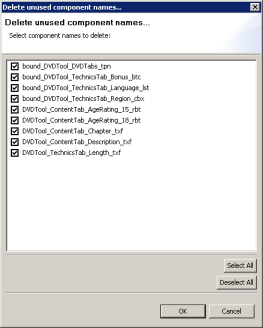
\includegraphics{52/ps/DeleteUnusedCompNames}
\caption{Deleting unused Component Names}
\label{RNDeleteUnusedCN}
\end{center}
\end{figure}
		
\end{itemize}

\textbf{HTML Test Result Reports can be expanded again}
\begin{itemize}
\item Following changes made for the initial contribution to Eclipse, the HTML Test Result Reports could not be viewed properly in the previous version. 
\item In this release, the nodes in the HTML reports can be expanded and collapsed to view the whole test progress. 

\begin{figure}[h]
\begin{center}
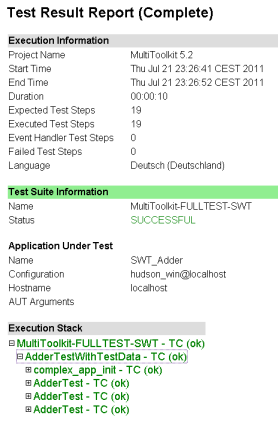
\includegraphics{52/ps/HTMLReport}
\caption{HTML Reports}
\label{RNHTMLReport}
\end{center}
\end{figure}
		
\end{itemize}

\textbf{State of component recognition displayed when collecting technical names}
\begin{itemize}
\item When a component (technical name) is collected from an \gdaut{}, it receives a colored
dot corresponding to the accuracy of the object recognition for this component \textit{at the time of collecting}.
\begin{description}
\item [A green dot]{signifies that the component could be found with an exact match, and was the only component above the threshold}.
\item [A yellow dot]{means that the component is an exact match, but that multiple other components were also above the threshold.}
\item [A red dot]{ means that this component cannot be relocated in the current state of the \gdaut{}}
\end{description}
\item As a side effect, the colors on the component names (green) and technical names (red) that were displayed in previous versions are now no longer shown. Once the \gdomeditor{} has been saved, all names are shown with plain black icons. 
\begin{figure}[h]
\begin{center}
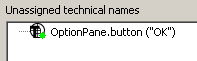
\includegraphics{52/ps/ColorDot}
\caption{Colored Dots for Object Mapping}
\label{RNColorDot}
\end{center}
\end{figure}
\end{itemize}

\textbf{Migration wizard re-enabled}
\begin{itemize}
\item  When migrating to the new version of \app{}, the migration assistant will automatically notify you that your database scheme is out-of-date. 
\item You can then select which \gdprojects{} to import (these must have been exported from the \gddb{} prior to migrating!).
\item The assistant will drop the tables in the \gddb{}, recreate the necessary tables and import the \gdprojects{} you specified.

\begin{figure}[h]
\begin{center}
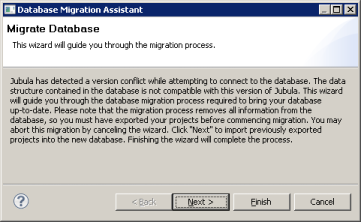
\includegraphics{52/ps/Migration}
\caption{Migration Wizard}
\label{RNMigration}
\end{center}
\end{figure}

\end{itemize}

\textbf{The DBTool is more verbose}
\begin{itemize}
\item The command line tool to import, export and delete \gdprojects{} in the \gddb{}, the DBTool, has been updated so that it is more verbose.
\end{itemize}

\textbf{Progress View}
\begin{itemize}
\item The \ite{} now  uses the progress view to show longer-running activities such as test execution, connecting to \gdauts{} etc.
\end{itemize}

\textbf{Edit Parameters Dialog in \gddataeditor{} can be opened via double-click}
\begin{itemize}
\item In the \gddataeditor{}  it is no longer necessary to open the Edit Parameters Dialog via context-menu, as it can now also be opened via double-click on the data set you wish to edit.
\end{itemize}


\textbf{Mac keyboards now supported, new mechanism for adding keyboard layout files}
\begin{itemize}
\item In the \gdaut{} configuration dialog for SWT and RCP \gdauts{}, 
\end{itemize}
